\documentclass[a4paper, 12pt]{report}
\usepackage{cmap} % поиск в PDF
\usepackage[T2A]{fontenc} % Кодировка
\usepackage[utf8]{inputenc} % Кодировка исходного текста
\usepackage[english,russian]{babel} % Локализация и переносы
\pagestyle{plain} % Для обозначения страниц справа снизу

\usepackage{graphicx}
\graphicspath{ {./images/} }

% Основная часть
\author{Автор: Булат Насыров}
\title{RFT\_CS \\ \footnotesize{\textit{Rocket fuel and trajectory computing system}}}
\date{\today}


\begin{document}
\maketitle

\tableofcontents{}
\clearpage
{\bfseries\Huge Предисловие}\\

\textrm{
    О чем будет идти речь, когда будем обсуждать ПО?\\
    Так же как любая метафора, описание программного обеспечения с точки зрения архитектуры может что-то скрыть, а что-то, наоборот, проявить; может обещать больше, чем давать, и давать больше, чем обещать. \\
    Оснавная привлекательность архитектуры - это структура. А структура - это то, что доминирует над парадигмами и суждениями в мире разработки ПО - компонентами, классами, функциями, модулями, слоями и службами, микро или макро. Но макроструктура многих программных систем часто пренебрегает убеждениями или пониманием - организация советских предприятий, невероятные небоскребы-башни (манареты) Дженга, достигающие облаков, археологические слои, залегающие в горной породе. Структура ПО не всегда интуитивно очевидна, как структура зданий.
}

\chapter{Введение}
\section{Концепция}
\textrm{
    RFT\_CS (Rocket fuel and trajectory computing system) Система расчета ракетного топлива и траектории полета ракеты - это Python-библиотека для разработки математических моделей. RFT\_CS изначально был спроектирован так, чтобы его можно было внедрять постепенно. Другими словами, \textbf{вы можете начать с малого и использовать только ту функциональность RFT\_CS, которая необходима вам в данный момент}. Также в случае, если вам нужно изменить поведение/вычисления функции, есть возможность конфигурации методов под ваши нужды.
}
\section{Цель}
\textrm{
    Основная цель - создать математическую модель процессов, связанных с полётом одно и многоступенчатых, твердо и жидко топливных ракет и для вычисления траектории полёта баллистических ракет. Данное ПО может быть использовано для создания космических/баллистических ракет или своих научных экспериментов.
}
\section{Технологии}
\textrm{
    Программное обеспечение построено на высокоуровневом языке программирования Python и отдельные микропроцессоры написаны на языке C. Также для сложных математических вычислений использовались библиотеки, специально созданные для этой цели.
}
\clearpage

\section{Декомпозиция задачи}
\textrm{
    Начнём с составных частей ракеты, а также внешние факторы, влияющие на полёт. Начнём с состава космической ракеты:
}

\begin{figure}[!ht]
\centering
\begin{subfigure}
    \centering
    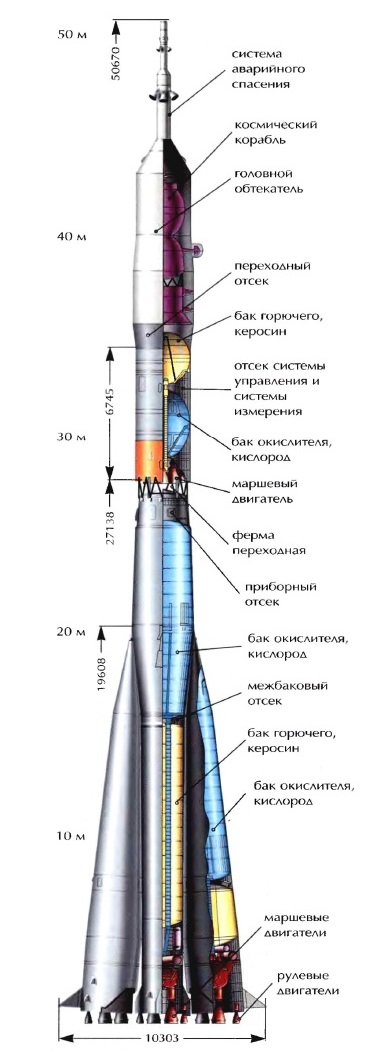
\includegraphics[width=.3\linewidth]{пример_космической_ракеты}
    \label{Рис. 1. Состав космической ракеты}
\end{subfigure}
\begin{subfigure}
    \centering
    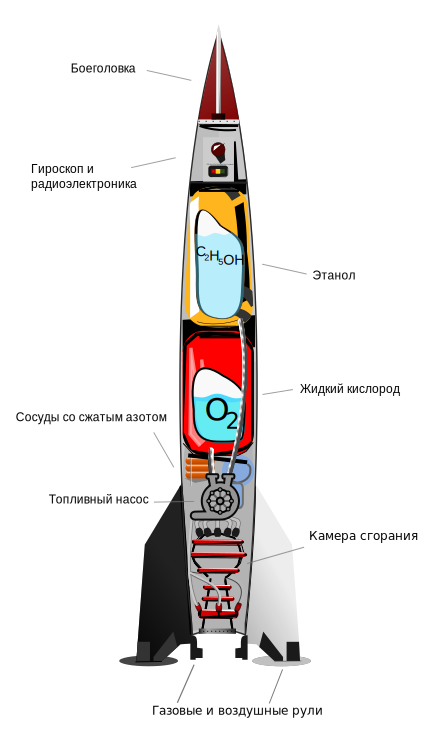
\includegraphics[width=.4\linewidth]{пример_баллистической_ракеты}
    \label{Рис. 2. Состав баллистической ракеты}
\end{subfigure}
\end{figure}

\section{Обработка ошибок}
\textrm{
    Могут возникать ошибки связанных с некорректным математических операций, перегрузкой или долгим ожиданием ответа от системы и неверным вводом/выводом данных, и др. Подобные ошибки обрабатываются и выводятся в виде ответа, а также записываются в логи. \bfseries {"При добавлении новых функций или использование встроенных функций важно не забывать обрабатывать ошибки и добавлять логирование для дальнейшего удобства исправления багов."}
}
\clearpage

\end{document}

